%% LyX 2.2.1 created this file.  For more info, see http://www.lyx.org/.
%% Do not edit unless you really know what you are doing.
\documentclass[english]{article}
\usepackage[T1]{fontenc}
\usepackage[latin9]{inputenc}
\usepackage{amsmath}
\usepackage{graphicx}

\makeatletter
%%%%%%%%%%%%%%%%%%%%%%%%%%%%%% User specified LaTeX commands.
\usepackage{cite}
\usepackage[T1]{fontenc}
\usepackage{inputenc}
\usepackage{authblk}
\usepackage{lmodern}
\author[1,2]{Daniel Schlauch} 
\author[1]{Joseph Paulson}
\author[2,3]{Kimberly Glass} 
\author[1,3]{John Quackenbush}
\affil[1]{Department of Biostatistics and Computational Biology, Dana-Farber Cancer Institute and Department of Biostatistics, Harvard TH Chan School of Public Health, Boston, MA 02115}
\affil[2]{Channing Division of Network Medicine, Brigham and Women's Hospital, Boston, MA 02115}
\affil[3]{Department of Medicine, Harvard Medical School, Boston, MA 02115}
\affil[4]{Pulmonary and Critical Care Division, Brigham and Women's Hospital and Harvard Medical School, Boston, USA}

\makeatother

\usepackage{babel}
\begin{document}

\title{Batch effect on covariance structure confounds network analyses in
gene expression studies}
\maketitle
\begin{abstract}
Systemic biases associated with multiple batches of gene expression
experiments have been known to confound results in differential gene
expression analyses. Numerous methods have been developed over the
past 10 years which address this phenomenon. Commonly, these approaches
correct expression values such that the mean and variance of each
gene is conditionally independent of a set of batch covariates. However,
methods published to date have not addressed potential differential
covariance across batches. While this is of lesser concern in the
context of standard differential gene expression, analyses that utilize
a gene co-expression or a correlation matrix will continue to see
confounding due to batch effect even after application of standard
batch-correction methods. In this article, we demonstrate the persistence
of confounding at the covariance level after standard batch correction
using simulation studies and real world examples. Finally, we present
an approach for computing a corrected gene expression coexpression
matrix, called {[}NAME{]}, based on a maximum likelihood estimation
of the conditional covariance matrix.
\end{abstract}

\section{Introduction}

While the accessibility of high-throughput assays has increases, so
too has the ability to investigate numerous hypotheses simultaneously. 

\textbf{{[}Continue babbling about basic experimental design of gene
expression studies...{]}}

Biological sources of variation are typically of interest, but observed
variation is often the result of technical artifacts which may confound
associations between experimental groups and gene expression. We can
assume the model $G_{ij}=\alpha_{j}+X\beta_{j}+B\gamma_{ij}+\delta_{ij}\epsilon_{ij}$,
where $G_{ij}$ is the gene expression of gene $j$ for sample $i$,
$X$ is the design matrix, $\beta_{j}$ is a vector of regression
coefficients for gene $j$ for the columns of $X$. The next two terms
specify the additive and multiplicative impacts of batch. \textbf{$B$}
is an matrix of indicators for each of the batches, and $\gamma_{j}$
is a vector of additive batch effects on gene $j$. $\epsilon_{ij}$
is the $N\left(0,\sigma_{j}^{2}\right)$ error term and $\delta_{ij}$
is the multiplier of that error term. Controlling for batch necessarily
involves estimating the impact of batch on the mean expression and
the variance of that expression, specifically $\gamma_{ij}$ and $\delta_{ij}$,
for each gene. Many steps of experimental protocols have been shown
to lead to batch effects, but it is generally not known what mechanism
is at fault for a particular study. Therefore it is typical to estimate
$\gamma_{ij}$ and $\delta_{ij}$ for each gene in a study., \textbf{{[}Continue
to describe general batch effect...{]}}

Despite widespread literature published regarding the identification
and control of confounding due to batch effect {[}citations{]}, batch
effect correction has focused on adjusting for the effects of batch
on gene expression mean and variance at an individual level. For example,
ComBat uses an empirical bayes approach to estimate the mean and variance
parameters for each gene and then computes an adjusted gene expression
which controls for these effects. However, in the context of network
inference, we are often interested in the covariance of genes as opposed
to marginal distribution of each gene. Essentially, we assume that
genes which are functionally related will exhibit a correlated expression
pattern across a set of experimental conditions or samples. 

Standard batch correction approaches fail to remove the impact of
a type of batch effect which may manifest itself by causing a differential
co-expression patterns between two or more genes. Removing the impact
of differential means and variances across batches is critical to
removing differential covariance across batch, but will be insufficient
if the covariance itself is associated with batch. While the impact
of this oversight may be negligible for differential gene expression
analysis, co-expression patterns are widely considered in the field
of network inference. The impact of confounding due to differential
coexpression in batches remains unexamined.

\textbf{{[}Describe recent work with sparse covariance estimation...{]}}

\section{Methods}

\subsection{Approach}

The conventional batch correction model is typically given as
\[
Y_{g}=\alpha_{g}+\beta_{g}X+\gamma_{i}gZ+\delta_{i}g\epsilon_{i}g
\]

where $X$ is the exposure (e.g. treatment/control) and $Z$ is the
batch (or other covariates). In the context of network inference,
we often want to find $cor(Y_{g1},Y_{g2})$, independent of $Z$. 

So, in order to model 2nd order batch, what we really want to do is
allow for the parameter of interest, $\beta_{g}$ to vary by batch.
So, now we set

$\beta_{g}^{*}=\beta_{g}+\beta_{B}gZ$

Where $\beta_{B}$ is a new parameter that we need to estimate for
each of the ${p \choose 2}$ comparisons.

We can write out a full model for any two genes. Note that $Y_{g2}$
is another gene in this model.

\[
Y_{g2}=\alpha_{g}+\beta_{g}^{*}X+\gamma_{i}gZ+\delta_{i}g\epsilon_{i}g
\]

or

\[
Y_{g2}=\alpha_{g}+(\beta_{g}+\beta_{B}gZ)X+\gamma_{i}gZ+\delta_{i}g\epsilon_{i}g
\]
 
\[
Y_{g2}=\alpha_{g}+\beta_{g}X+\beta_{B}gZX+\gamma_{i}gZ+\delta_{i}g\epsilon_{i}g
\]

There are many ways to approach this, but I believe the best way is
the following steps:

1. Apply conventional batch correction. This will effectively eliminate
the $\gamma_{i}gZ$ term and we can proceed with the simpler model
- 
\[
Y_{g2}=\alpha_{g}+\beta_{g}X+\beta_{B}ZX+\delta_{i}g\epsilon_{i}g
\]
 - on the combat-corrected data. Further standardize each gene expression
(this will not impact the actual results, but will aid in interpretation
and computation time)

2. Fit the following models Reduced: 
\[
Y_{g2}=\alpha_{g}+\beta_{g}X+\delta_{i}g\epsilon_{i}g
\]
 Full: 
\[
Y_{g2}=\alpha_{g}+\beta_{g}X+\beta_{B}ZX+\delta_{i}g\epsilon_{i}g
\]

3. Place estimated coefficients into two separate matrices (
\[
S_{\beta},S_{B}
\]
). We have tons of options for computing these coefficients. A LASSO-style
L1 regularization would probably make the most sense here, but for
the purposes of simplicity we will start with OLS.

So, now we have two separate (equal sized) matrices instead of the
usual one. $S_{\beta}$ is the estimated similarity matrix and $S_{B}$
is the \textquotedbl{}batch impact\textquotedbl{}. Intuitively, we
can imagine that the expected value of $S_{B}$ is a zero matrix in
the absence of 2nd order batch effects. This lends itself easily for
2nd order batch effect testing - for example, we can compare the two
models via likelihood ratio test (LRT). This is nice, but we're much
more interested in 2nd order batch effect {*}correction{*}.

4. Compute the corrected similarity matrix via: 
\[
\hat{S_{i}^{*}}=\hat{S_{\beta}}+(\frac{\sum_{j\in X_{i}}Z_{j}}{n_{i}})\hat{S_{B}}
\]

This yields a similarity matrix that is {*}{*}batch-independent{*}{*}.
In other words, we can now compare networks computed with different
proportions of batch membership. We can think of the adjusted similarity
matrix as being the estimated similarity matrix given a {*}standardized
representation of batches{*}. This standardization allows us to compare
networks which have been inferred with differing batch composition.

Obviously, the usual caveats apply - this correction is most useful
when the batches in each exposure are (a) unequal, (b) not too unequal.
Small numbers of samples for batches will result in wild fluctuations
in terms of estimating batch effect. 

\subsection{Model}

Consider a set of $N$ samples with $q$ covariates measuring gene
expression across $p$ genes. Let $\textbf{x}_{i}=(x_{i1},\dots,x_{iq})$
denote the confounding covariates for sample $i$ and let $\textbf{g}_{i}=(g_{i1},\dots,g_{ip})$
denote the gene expression values for sample $i$ for the $p$ genes.

In multivariate regression form we can express this as 
\[
\textbf{g}_{i}=\mathbf{\beta}^{T}\textbf{x}_{i}+\mathbf{\epsilon}_{i}\text{ for }i=1,\dots,N
\]
 where $\mathbf{\beta}$ is a $q\times p$ matrix of coefficients.

Equivalently,

\[
\textbf{G}=\textbf{X}\mathbf{\beta}+\mathbf{E}
\]

where $\textbf{G}$, $\textbf{X}$, and $\textbf{E}$ are each matrices
with row $i$ corresponding to $\textbf{g}_{i}$, $\mathbf{x}_{i}$,
and $\mathbf{\epsilon}_{i}$ respectively.

Here, we make the usual multivariate assumption for $\textbf{E}$
that the rows $\mathbf{\epsilon}_{i},\dots,\mathbf{\epsilon}_{N}$
are independent, and follow distribution, $MVN_{p}(\mathbf{0},\Sigma_{i})$.
Notably in this paper, the covariance of $\mathbf{\epsilon}_{i}$
differ according to $i$.

Estimating the covariance structure for a set of $p$ genes typically
involves computing the sample covariance matrix, $S$, with entries
$s_{jk}=\frac{1}{N-1}\sum_{i=1}^{N}(G_{ij}-\bar{G_{\cdot j}})(G_{ik}-\bar{G_{\cdot k}})$.
However, as is typical in high-throughput settings, $p\gg N$, producing
an estimated covariance matrix $p\times p$ with column rank $\le N$.

To address this \textquotedbl{}curse of dimensionality\textquotedbl{},
numerous methods have been proposed. One might use a series of LASSO
regressions to estimate parameters in the inverse covariance matrix
{[}Meinshausen \& Buhlmann (2006){]}, or perform penalized maximum
likelihood estimation with the penalty on the inverse covariance matrix{[}Yuan
\& Lin (2007), Friedman (2007), Banerjee (2008){]}. Each of these
approaches imposes sparsity on the precision matrix, effectively assuming
a large degree of conditional independence between genes. More recent
work has explored imposing sparsity on the covariance matrix itself,
rather than the precision matrix {[}Bien \& Tibshirani 2011{]}, which
allows us to assume widespread marginal independence of genes. 

The approach we take here involves estimating a covariance matrix
$\Sigma_{i}$ which depends on the batch and experimental design features
of sample $i$. An estimate of $\Sigma_{i}$ which allows all elements
of the matrix to vary freely can be obtained by separately estimating
the covariance matrix for each unique row of $\mathbf{X}$. However,
this approach in impractical for a large number of categorical covariates
or any continuous covariates. Given that genes often behave in distinct
patterns, it is inefficient to estimate coexpression values for every
pairwise combination of genes.

Instead, we approach the problem by making use of the fact that genes
commonly behave in coexpressed modules, and that the dimensional space
is effectively much smaller than $p^{2}$. To do this, we decompose
the gene expression correlation matrix and find a set of eigenvectors
which explain the variation. We then attempt to infer a diagonal matrix
of pseudo-eigenvalues, which maximize the likelihood function below.
This procedure allows us to reduce the parameter space from $p^{2}$
to $p$ or less while still considering the bulk of the variability
in the data.

Instead of estimating all entries in the covariance matrix, $\Sigma_{i}$,
we instead estimate $\hat{\Sigma_{i}}=\mathbf{Q}\mathbf{\Lambda}^{\left(i\right)}\mathbf{Q}^{T}$,
where $\mathbf{Q}$ is held constant as the set of eigenvectors from
the full covariance matrix. In this formulation,$\mathbf{\Lambda}$
is a diagonal matrix with entries 
\begin{equation}
\mathbf{\Lambda}_{kk}^{\left(i\right)}=\mathbf{X}_{i}\mathbf{\gamma}_{\cdot k}\label{eq:Lambda_diag}
\end{equation}
 where $\mathbf{X}$ is the covariate matrix and$\mathbf{\gamma}$
is a $q\times p$ matrix of coefficients. 

Let $M_{j}$ be a $p\times p$ matrix with $1$ at position $\left(j,j\right)$
and 0 at all other positions and let $\mathbf{v}_{j}$ be a $p-vector$
of 0s except for a 1 at position $j$. Also, let $q$ be a positive
integer with $q\le p$. We can express $\mathbf{\Lambda}^{\left(i\right)}$
as
\begin{equation}
\mathbf{\Lambda}^{\left(i\right)}=\sum_{j=1}^{q}M_{j}\mathbf{X}_{i}\mathbf{\gamma}\mathbf{v}_{j}^{T}\label{eq:Lambda}
\end{equation}
The value taken with $q$ specifies the number of pseudo-eigenvalues
which are to be estimated. It is straightforward to show that in the
case of a single batch, where $\mathbf{X}=\mathbf{1}_{N}$, and with
$q=p$,$\mathbf{\gamma}$ becomes the vector of eigenvalues from the
original covariance matrix.

\subsection{Likelihood function}

The likelihood function is 
\[
\mathcal{L}\left(\mu,\Sigma\right)=\prod_{i=1}^{N}\frac{1}{\left(2\pi\right)^{\frac{p}{2}}|\Sigma_{i}|^{\frac{1}{2}}}e^{-\frac{1}{2}\left(\mathbf{G}_{i}-\mu\right)^{T}\Sigma_{i}^{-1}\left(\mathbf{G}_{i}-\mu\right)}
\]

The maximum likelihood estimation of $\mathbf{\mu}$ is simply the
vector $\mathbf{\bar{g}}=\frac{\sum_{i=1}^{N}\mathbf{g}_{i}}{N}$,
so we can plug in that estimate into the likelihood

\[
\mathcal{L}\left(\Sigma\right)=\prod_{i=1}^{N}\frac{1}{\left(2\pi\right)^{\frac{p}{2}}|\Sigma_{i}|^{\frac{1}{2}}}e^{-\frac{1}{2}\left(\mathbf{G}_{i}-\mathbf{\bar{g}}\right)^{T}\Sigma_{i}^{-1}\left(\mathbf{G}_{i}-\mathbf{\bar{g}}\right)}
\]
and the log-likelihood is:
\[
log\mathcal{L}\left(\Sigma\right)\propto\sum_{i=1}^{N}log\left(det\left(\Sigma_{i}\right)^{\frac{-1}{2}}\right)+\sum_{i=1}^{N}-\frac{1}{2}\left(\mathbf{G}_{i}-\mathbf{\bar{g}}\right)^{T}\Sigma^{-1}\left(\mathbf{G}_{i}-\mathbf{\bar{g}}\right)
\]

Without loss of generality, we may center the expression matrix, $\mathbf{G}$,
by subtracting off the means, such that $\mathbf{G}_{i}^{*}=\mathbf{G}_{i}-\mathbf{\bar{g}}$.
And substituting the expanded version of $\mathbf{Q}\mathbf{\Lambda}^{\left(i\right)}\mathbf{Q}^{T}$

\begin{align*}
log\mathcal{L}\left(\mathbf{\gamma}\right) & \propto\frac{-1}{2}\sum_{i=1}^{N}log\left(det\left(\mathbf{Q}\sum_{j=1}^{q}\left[M_{j}\mathbf{X}_{i}\mathbf{\gamma}\mathbf{v}_{j}^{T}\right]\mathbf{Q}^{T}\right)\right)\\
 & -\frac{1}{2}tr\left[\left(\mathbf{Q}\sum_{j=1}^{q}\left[M_{j}\mathbf{X}_{i}\mathbf{\gamma}\mathbf{v}_{j}^{T}\right]\mathbf{Q}^{T}\right)^{-1}\sum_{i=1}^{N}\mathbf{G}_{i}^{*T}\mathbf{G}_{i}^{*}\right]
\end{align*}

Differentiating with respect to $\gamma$ yields
\begin{align*}
d\,log\mathcal{L}\left(\mathbf{\gamma}\right) & =\frac{-1}{2}\sum_{i=1}^{N}tr\left(\mathbf{Q}\sum_{j=1}^{q}\left[M_{j}\mathbf{X}_{i}\mathbf{\gamma}\mathbf{v}_{j}^{T}\right]\mathbf{Q}^{T}\right)^{-1}d\gamma\\
 & -\frac{1}{2}tr\left[-\sum_{i=1}^{N}\left(\mathbf{Q}\sum_{j=1}^{q}\left[M_{j}\mathbf{X}_{i}\mathbf{\gamma}\mathbf{v}_{j}^{T}\right]\mathbf{Q}^{T}\right)^{-1}d\gamma\left(\mathbf{Q}\sum_{j=1}^{q}\left[M_{j}\mathbf{X}_{i}\mathbf{\gamma}\mathbf{v}_{j}^{T}\right]\mathbf{Q}^{T}\right)^{-1}\mathbf{G}_{i}^{*T}\mathbf{G}_{i}^{*}\right]\\
\end{align*}
 To find the maximum, we set $d\,log\mathcal{L}\left(\mathbf{\gamma}\right)=0$.
This is satisfied when
\begin{align*}
0 & =-\frac{1}{2}tr\left(\sum_{i=1}^{N}\left(\mathbf{Q}\sum_{j=1}^{q}\left[M_{j}\mathbf{X}_{i}\mathbf{\gamma}\mathbf{v}_{j}^{T}\right]\mathbf{Q}^{T}\right)^{-1}d\gamma\left(I_{p}-\sum_{i=1}^{N}\left(\mathbf{Q}\sum_{j=1}^{q}\left[M_{j}\mathbf{X}_{i}\mathbf{\gamma}\mathbf{v}_{j}^{T}\right]\mathbf{Q}^{T}\right)^{-1}\sum_{i=1}^{N}\mathbf{G}_{i}^{*T}\mathbf{G}_{i}^{*}\right)\right)\\
\end{align*}
This is satisfied when the right term is 0, or when 
\[
\sum_{i=1}^{N}\left(\mathbf{Q}\sum_{j=1}^{q}\left[M_{j}\mathbf{X}_{i}\mathbf{\gamma}\mathbf{v}_{j}^{T}\right]\mathbf{Q}^{T}\right)=\sum_{i=1}^{N}\mathbf{G}_{i}^{*}\mathbf{G}_{i}^{*T}
\]


\subsection{Corrected covariance matrix}

Given an estimate for $\gamma$, $\hat{\gamma}$, we can now estimate
the batch-independent covariance structure as 
\[
\hat{\mathbf{S}}=\bar{\mathbf{X}}\hat{\gamma}
\]
 where $\bar{\mathbf{X}}$ is a $q$-vector specifying the column
means of $\bar{\mathbf{X}}$,
\[
\bar{\mathbf{X}}=\frac{\sum_{i=1}^{N}\mathbf{x}_{i}}{N}
\]

Computing the differential covariance matrix between two conditions,
defined as column 2 of $\mathbf{X}$, can be performed via 
\[
\hat{\mathbf{W}}=\mathbf{y}\hat{\gamma}
\]
where $\mathbf{y}=\left(0,1,0,\dots0\right)$

\section{Results}

\subsection{Simulated Demonstration}

Consider a set of samples from a study involving two batches. Let
the expression data be distributed as a set of MVN with mean vector
$\mu$ and covariance structure $\Sigma$.

Existing batch correction methods are designed to identify differentially
expressed genes and thus focus on $\mu$ and the diagonal of $\Sigma$.

For network inference, however, we are less interested in these values
and more interesting in the off-diagonal of $\Sigma$. Mechanisms
for batch effect which act on the covariance structure rather than
the mean and variance structure will not be corrected for using existing
batch correction methods.

In Figure \ref{simulated_example}, we see two examples of uncorrected
batch effect (Left) impacting two genes in a study. In the top row,
batch effect alters the means and variances of the two genes. In the
bottom row, the means, variances \emph{and} coexpression is impacted.
Upon application of ComBat (Right) to the uncorrelated genes, the
two genes become independent as desired. However, when applied to
the conditionally coexpressed case (Bottom row) we continue to observe
differential coexpression across batches.

To demonstrate the general concept of how differential coexpression
leads to inflated test statistics, we simulated two studies, each
of 200 individuals across 10,000 genes. Each sample was a realization
of a multivariate normal distribution with $\mathbf{\mu}=\mathbf{0}_{p},$
and borrowed a coexpression matrix of 10,000 genes from an existing
dataset (ECLIPSE) to be $\mathbf{\Sigma}$. For Study 1, we sampled
200 times from this distribution. For Study 2, we sampled 150 times
using $\Sigma$, and then estimated a new $\Sigma^{*}$ using 9000
of the same genes from the ECLIPSE study, but with 1000 new genes.
This procedure was intended to mimic the introduction of newly active
biological pathways in a subset of the samples as we might expect
with batch effect. Our goal was to observe how the distribution of
the estimated coexpression matrix differed according to the different
covariance approaches. The results are seen in Figure 2, showing an
inflation of significant results... \textbf{{[}describe this in more
detail{]}}

Second order batch effect in GTEx clearly exists (see above), but
it can be subtle. For the purposes of a proof on concept, we can generate
a much stronger batch effect which clearly demonstrates this approach.
We simply select 5000 genes and 5000 separate genes in the other batch,
relabeling them Gene1, Gene2,\dots , Gene5000. Basically, we\textquoteright re
simply mismatching the genes between the batches! This, obviously,
causes a completely random rewiring of the network from one batch
to the other.

\begin{figure}
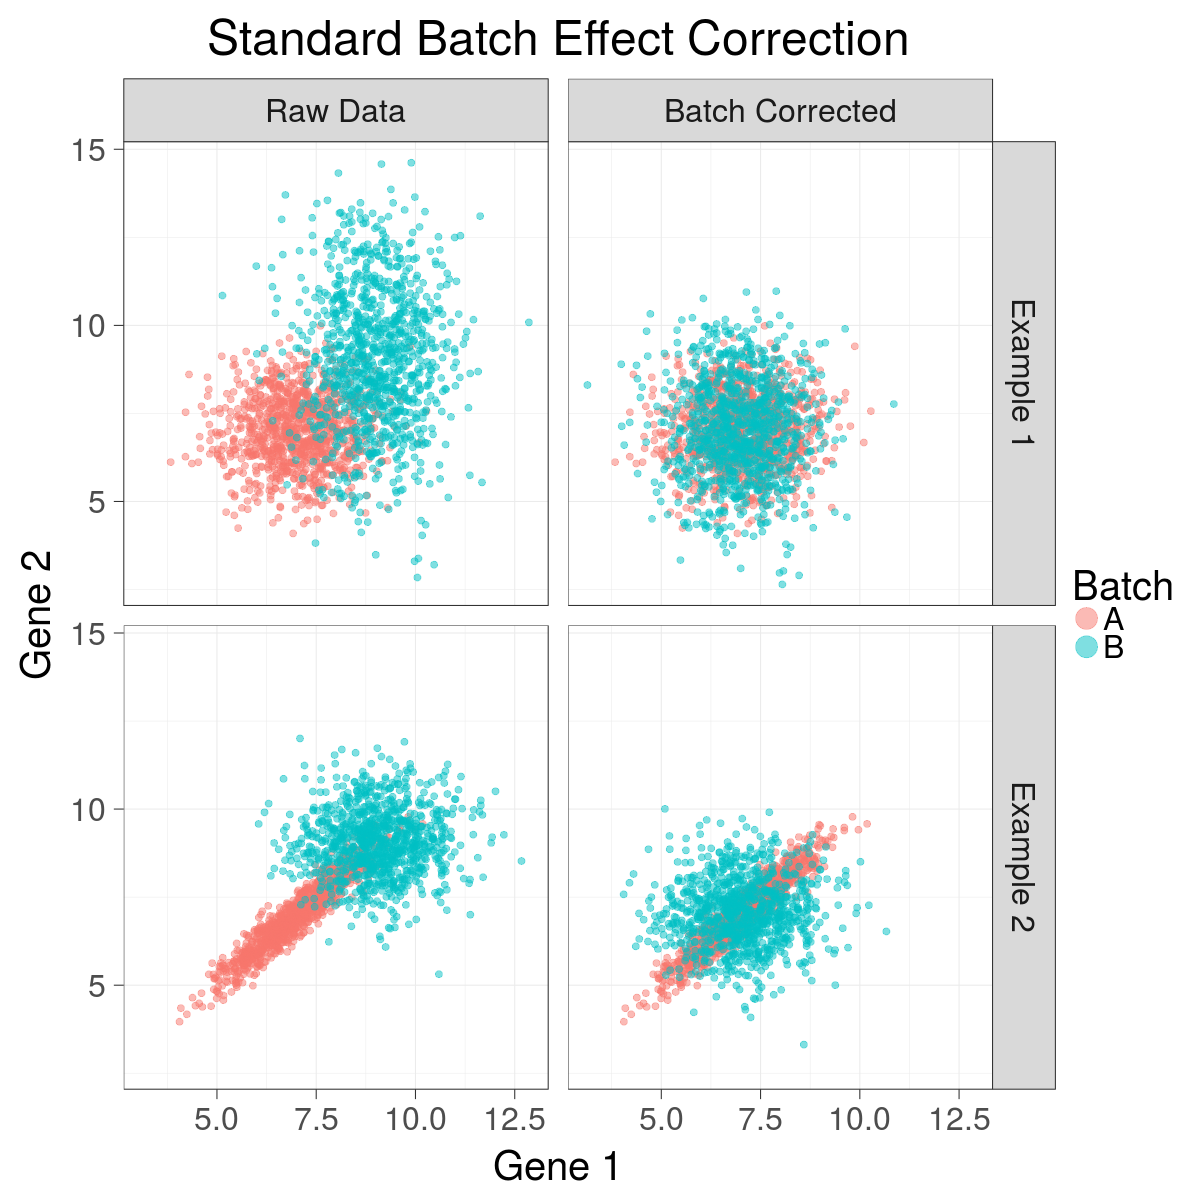
\includegraphics[width=1\columnwidth]{figures/simulated_example}\caption{Example of what works and doesn't work for batch effect}
\label{simulated_example}
\end{figure}

\begin{figure}
A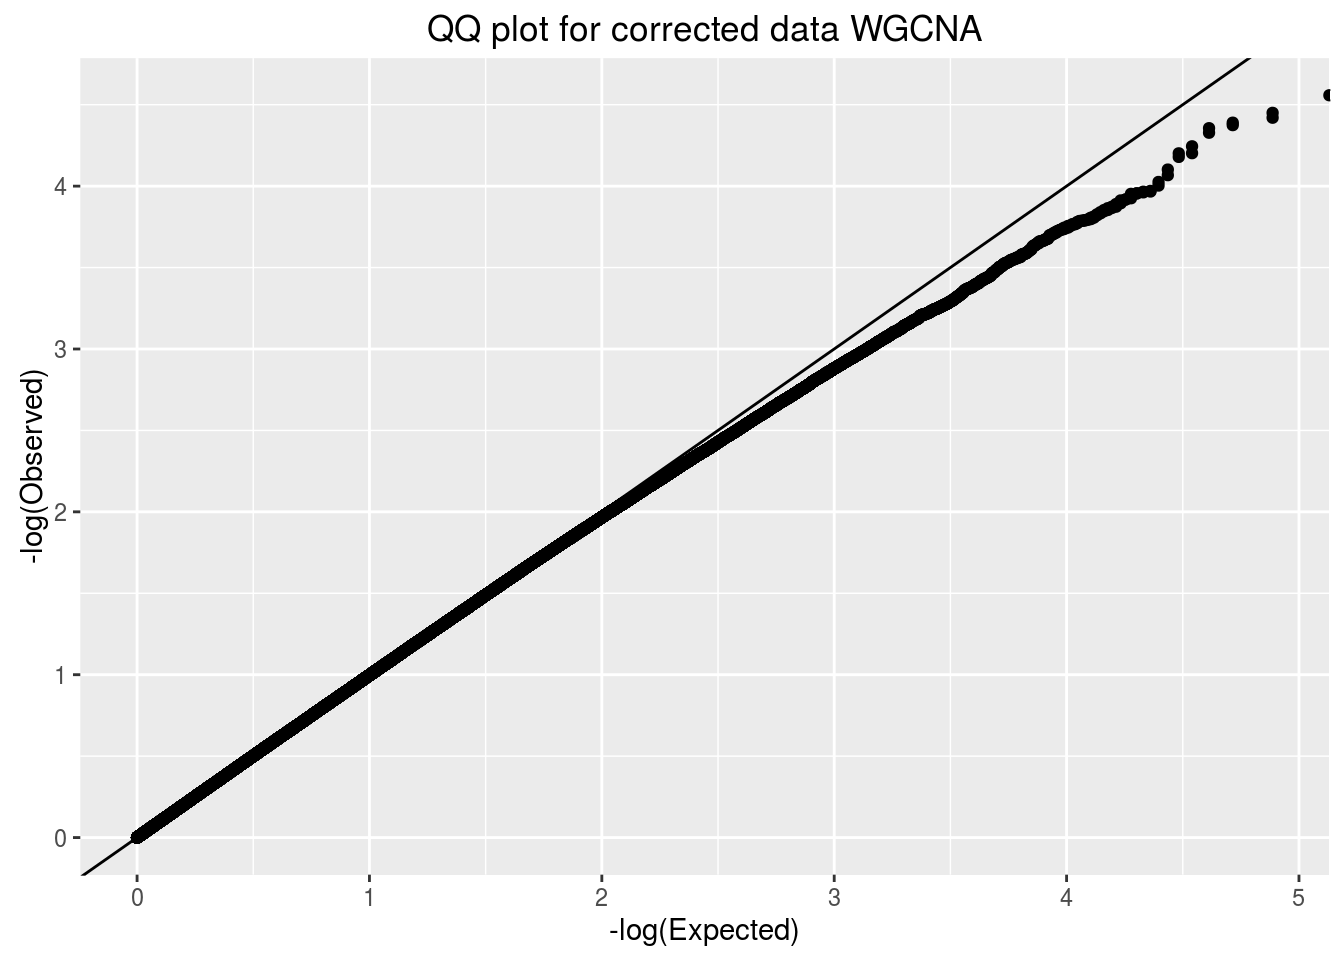
\includegraphics[width=0.4\columnwidth]{figures/pasted2}B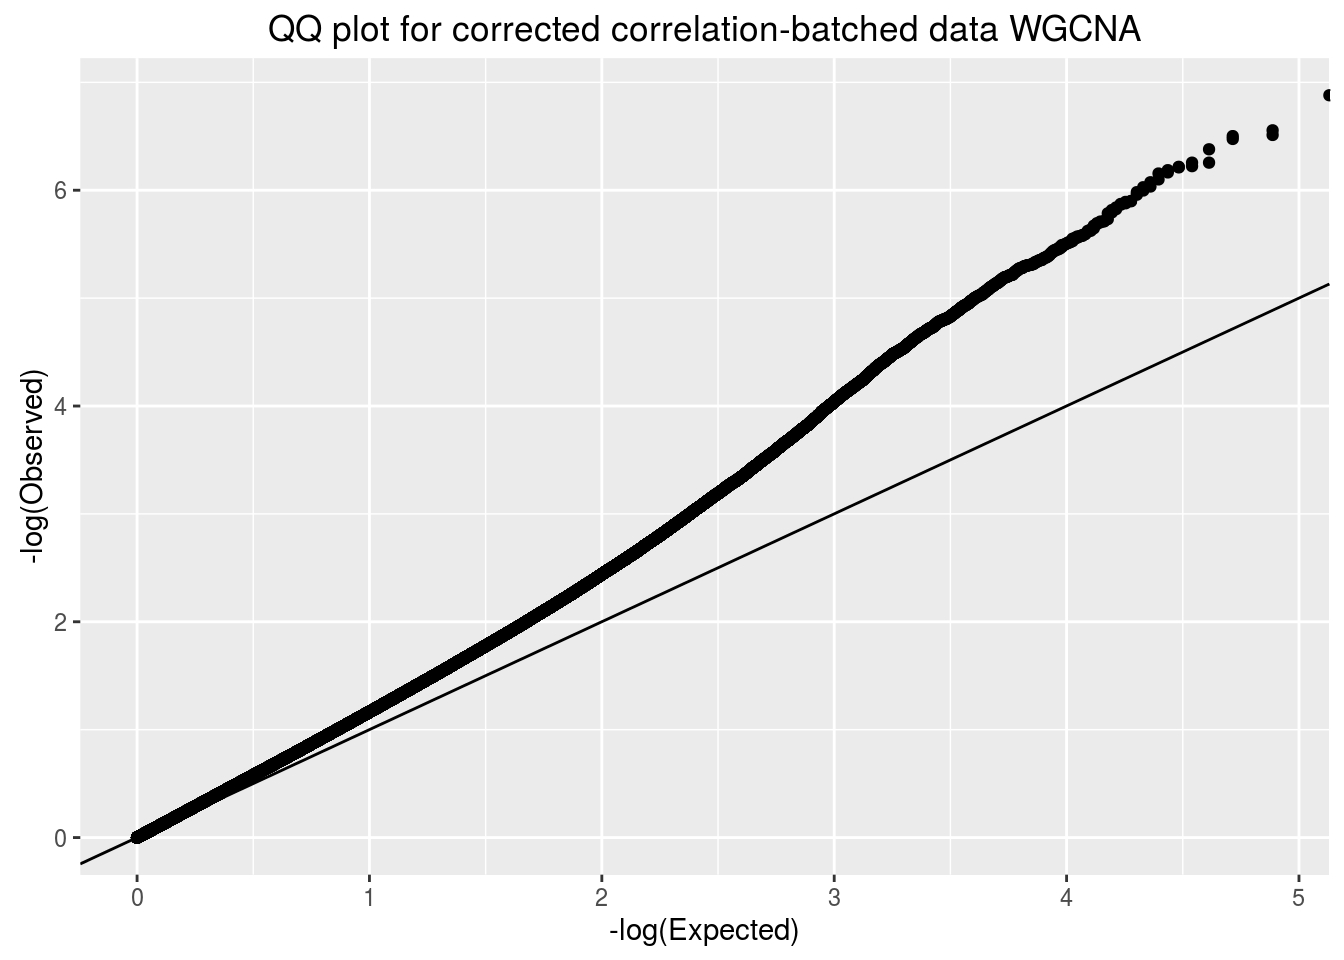
\includegraphics[width=0.4\columnwidth]{figures/pasted1}

\caption{QQ plots for simulated data without differential covariance (A) and
with differential covariance (B).}
\end{figure}


\subsection{Batch effect in GTEx Project}

GTEx uses WGCNA to find common modules across tissues. {[}Describe
GTEx{]}

GTEx Consortium uses state-of-the-art methods for attempting to adjust
for batch including study design and expression value correction.

Study design:

\emph{``To the extent possible, based on sample availability, batches
for library construction were designed to include a range of samples
from different tissues and to span multiple donors, so as to minimise
donor and tissue batch effects.''}

Expression correction:

\emph{``the effect of top 3 PEER factors, gender, and 3 genotype
PCs were removed.''}

However, neither of these address the \textquotedbl{}second order\textquotedbl{}
batch issue. These corrections inherently assume that batch affects
the location-scale distribution of gene expression independently and
thus does not consider the scenario where coexpression is the feature
impacted by batch.

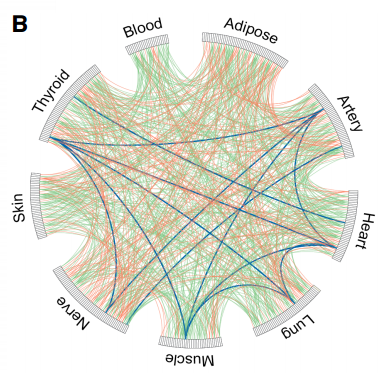
\includegraphics{figures/gtex_image}{[}GTEx Supplement{]} {[}Reproduce
this figure or remove it{]}

To demonstrate that this study is sensitive to batch, we choose two
widely available tissue types (Blood and Lung) from the data {[}YARN
normalization{]}.

We then apply batch correction using ``Center'' as the batch of
interest. We then ran WGCNA on each tissue separately as described
in {[}GTEx paper{]} and compute modules based on Topological Overlap
Map. 

We then ran the same procedure, but subsetted the data by each of
the 3 centers. In theory, after correcting for batch, the modules
observed should have been independent of the batch used to find them.
However, we observe dramatic (notable? clear?) differences in the
modules identified. We should really quantify this difference somehow.
This may require a clever resampling scheme where we select samples
both randomly and by center to measure variability.

\begin{figure}
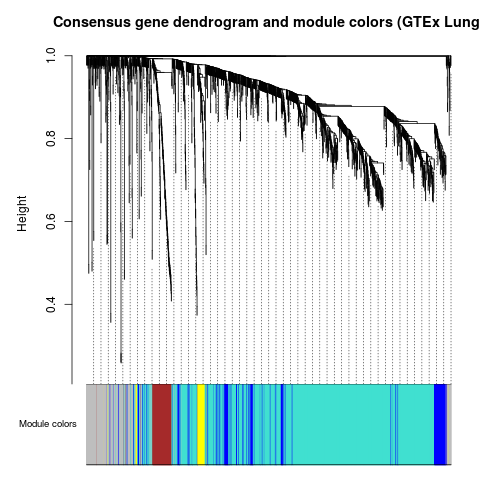
\includegraphics[width=0.4\columnwidth]{figures/pasted4}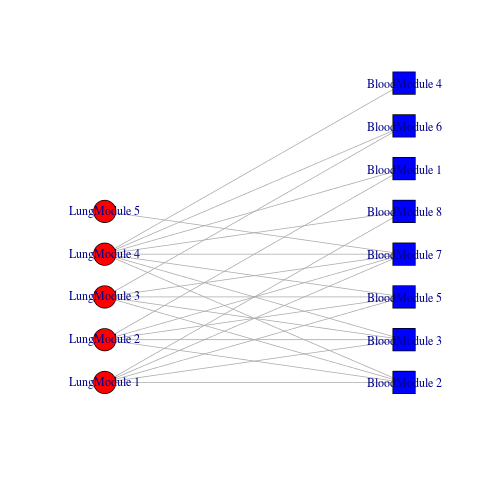
\includegraphics[width=0.4\columnwidth]{figures/pasted5}

A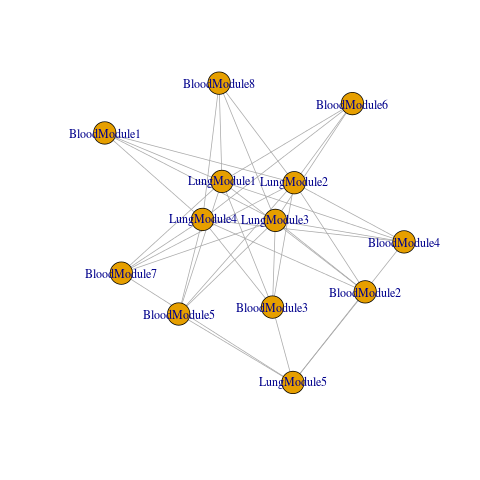
\includegraphics[width=0.3\columnwidth]{figures/pasted6}B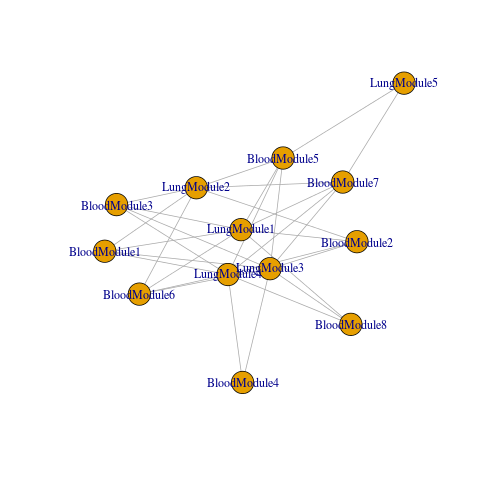
\includegraphics[width=0.3\columnwidth]{figures/pasted7}C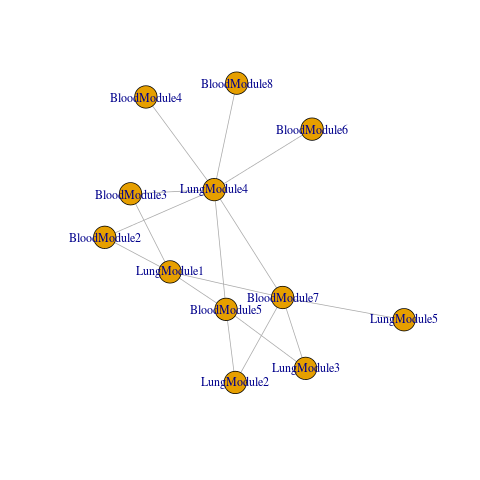
\includegraphics[width=0.3\columnwidth]{figures/pasted8}

\caption{Make these nicer. Combine into single plot? }
\end{figure}


\subsection{Confounding due to sex in ECLIPSE study}

In this analysis, we will perform a very common analysis: Build coexpression
networks based on \emph{COPD} vs \emph{Smoker control} and identify
consensus modules with WGCNA. \emph{Gender} is treated as a confounder,
but is only corrected using standard batch correction methods.

1. Run ComBat on gene expression data, {*}including gender as a covariate{*}. 

2. Sample a set of designs from this study which include varying degrees
of gender imbalance. 

3. Evaluate the agreement between cases and controls with pseudo-R\textasciicircum{}2
from multinomial logistic regression. 

4. Determine the degree to which the agreement between cases and controls
depends on the gender distribution.

While this data is reasonably balanced, we can use it to demonstrate
how sensitive our results are to confounding that was \emph{supposedly
}accounted for already. Figure \ref{AgreementVsConfounder}

\begin{figure}
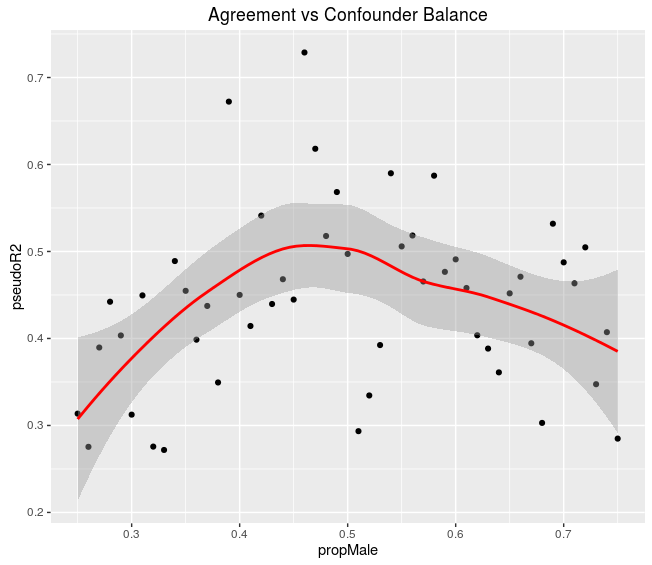
\includegraphics[width=1\columnwidth]{figures/pasted9}\caption{Very clear dependence of agreement between cases and control on the
balance. In other words, with a strong lack of balance, we see weaker
agreement, indicating that the results we DO see are a function of
the confounder and not the case-control partition.}

\label{AgreementVsConfounder}
\end{figure}


\section*{Discussion}

Thoughts about impact on any analysis involving coexpression with
batches...

Thoughts about generality of estimating covariance matrices in the
context of confounding.
\end{document}
